\section{误差与计算成本}
\label{sec:pdenum-error-cost}

一次计算结束后，怎样判断结果有多可信，又该把算力花在哪里？式~\eqref{eq:pdenum-error-split}把总误差分成了几段，这里逐段检验，再比较各种做法的代价。

\paragraph{用加密检查实际收敛}
真解已知时，比较相邻两层网格的误差，就得到\term{观测阶}（observed order）：
\begin{equation}
 p_{\mathrm{obs}}=\log_2\frac{E(h)}{E(h/2)} .
 \label{eq:pdenum-observed-order}
\end{equation}
表~\ref{tab:pdenum-fd-refine}和图~\ref{fig:pdenum-fd-rates}都是这样读出阶数的。真解未知时，有两种常用的办法。

第一种是构造解：先选一个光滑函数当作解，代入方程算出对应的源项和边值，再用这些数据检验程序。式~\eqref{eq:pdenum-model}就是这样得到的。这种办法检验的是程序和格式，不检验实际问题的解是否足够光滑。

第二种是比较三层网格。若误差的主项是$Ch^p$，相邻两层解的差的比值给出
\begin{equation}
 p_{\mathrm{obs}}\approx\log_2\frac{\lVert\bm{U}_h-\bm{U}_{h/2}\rVert}{\lVert\bm{U}_{h/2}-\bm{U}_{h/4}\rVert},
 \label{eq:pdenum-three-grid}
\end{equation}
这里的差要在公共节点上计算。它的前提是这几层网格已进入渐近范围，解的奇性、激波和未分辨的小尺度都可能破坏这一点。

\paragraph{分开估计各段误差}
只加密一个方向，就能把对应的误差段暴露出来。图~\ref{fig:pdenum-error-plateau}(a)解热方程，时间步固定为$\tau=0.05$时，加密空间网格到一定程度后误差停在约$7.7\times10^{-3}$，这就是时间误差的水平；$\tau=h$同步加密时，Crank--Nicolson方法的误差按$h^2$下降。

\begin{BookInlineFigure}
 \centering
 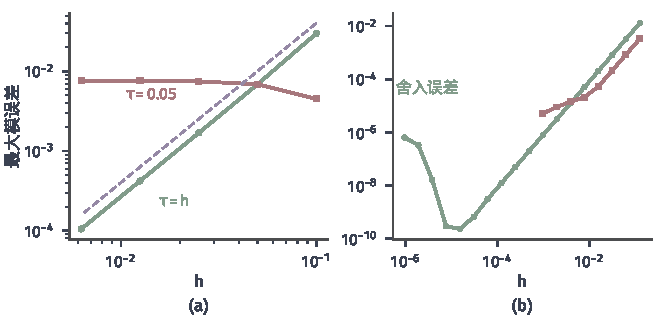
\includegraphics[width=112mm]{figures/06-differential-equations/02-partial-differential-equations/matplotlib/pdenum-error-plateau/figure.pdf}
 \caption{误差的停滞，紫色虚线是斜率$2$。(a)Crank--Nicolson方法解$u_0=\sin(\pi x)$的热方程到$T=0.1$：绿线$\tau=h$，红线固定$\tau=0.05$，后者被时间误差挡住。(b)一维Poisson问题：绿线用三对角消元直接求解，$h<2^{-16}$后舍入误差占主导；红线用共轭梯度法解$-u''=(3x+x^2)\mathrm{e}^x$，相对残差到$10^{-2}$就停止，加密后误差不再按$h^2$下降。}
 \label{fig:pdenum-error-plateau}
\end{BookInlineFigure}

积分误差也要单独看。第~\ref{sec:pdenum-assembly}小节中，同一个分片线性有限元，精确积分时节点误差为零，梯形积分时节点误差是$0.0530$，这份差别完全来自载荷的计算。

代数误差分两种。图~\ref{fig:pdenum-error-plateau}(b)的绿线是舍入误差：$\bm{A}_h$的条件数按$h^{-2}$增长，$h$小于$2^{-16}$后误差反而回升，最小值约为$2\times10^{-10}$。红线是迭代提前停止的误差：停止准则只控制残差，残差除以$\bm{A}_h$才是解的误差，所以固定的相对残差不能随网格加密自动提高解的精度。

一个实用的原则是让各段误差大致同一量级，多花的算力才有回报。迭代的容差应该随$h$收紧，时间步应该按格式的阶数跟着$h$减小。

\paragraph{计算成本}
设空间维数为$d$，每个方向的步长为$h$，未知量个数$N\sim h^{-d}$。差分和低阶有限元的矩阵每行只有常数个非零元，存储是$O(N)$。表~\ref{tab:pdenum-cost}比较了几种做法在单次求解或推进到固定时刻时的主要代价。

\begin{BookInlineTable}
 \centering
 \caption{$N\sim h^{-d}$个未知量时的代表性成本，$T$固定，常数和对数因子未写出。}
 \label{tab:pdenum-cost}
 \begin{tabular}{p{32mm}p{28mm}p{36mm}}
  \toprule
  做法 & 主要运算量 & 限制因素\\
  \midrule
  一维三对角消元 & $O(N)$ & 无\\
  带状消元，$d=2$ & $O(N^{2})$ & 带内填充，存储$O(N^{3/2})$\\
  共轭梯度，不预条件 & 约$O(N/h)$ & 迭代数随$\kappa^{1/2}\sim h^{-1}$增长\\
  显式扩散，$\tau\sim h^2$ & $O(N/h^2)$ & 稳定性\\
  隐式扩散，$\tau\sim h$ & $O(1/h)$次线性求解 & 每步的求解成本\\
  显式守恒格式，$\tau\sim h$ & $O(N/h)$ & CFL条件\\
  \bottomrule
 \end{tabular}
\end{BookInlineTable}

显式和隐式的取舍随问题而变。扩散问题的稳定性要求$\tau\sim h^2$，网格加密时显式方法的步数增长得很快，隐式方法每步更贵，但步数少得多。双曲问题的时间尺度本来就是$h$量级，显式格式的步长限制几乎不造成浪费，隐式方法反而难以获益。

大规模线性方程组的求解不在本章展开，可参考\BookChapterRef{chap:krylov-methods}{卷二第15章“Krylov子空间法”}；非线性问题每步的Newton迭代可参考\BookChapterRef{chap:second-order-methods}{卷五第7章“二阶方法”}。这些内层迭代的容差都属于式~\eqref{eq:pdenum-error-split}的最后一段。

还要记住，这些成本比较都建立在解的光滑性假设上。有激波或奇性时，全局加密的效率很低，图~\ref{fig:pdenum-fem-rates}(b)的加密网格只增加了靠近奇点的分辨率，就把一阶收敛恢复了回来。
